\documentclass[a4paper, 12pt]{article}
\usepackage[top=2cm, bottom=2cm, left=2.5cm, right=2.5cm]{geometry}
\usepackage[utf8]{inputenc}
\usepackage{graphicx}
\usepackage{subfig}
\usepackage[brazil]{babel}

\title{Simulação de Valores Pseudo-Aleatórios e Quasi-Aleatórios \\
\large Laboratório de Computação(MAP 2212)}
\author{Fabio Carvalho de Souza Nº USP 9425125 \\ 
Instituto de Matemática e Estatistica- IME}


\begin{document}

\maketitle

   A proposta do segundo exercício tem como objetivo propor uma maneira de dizer o quão evidente é a variabilidade de ocorrências de valores aleatórios dentro do intervalo [0,1]x[0,1] considerando valores pseudo aleatórios e quasi-aleatórios.
  \begin{figure}[h]
  \centering
  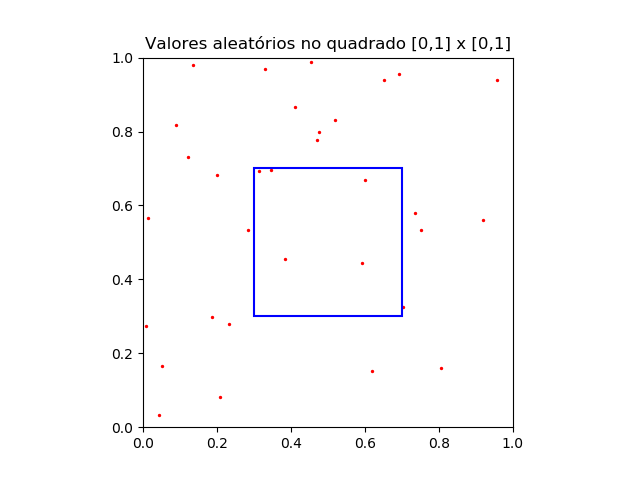
\includegraphics[scale=0.35]{32pseudo.png}
  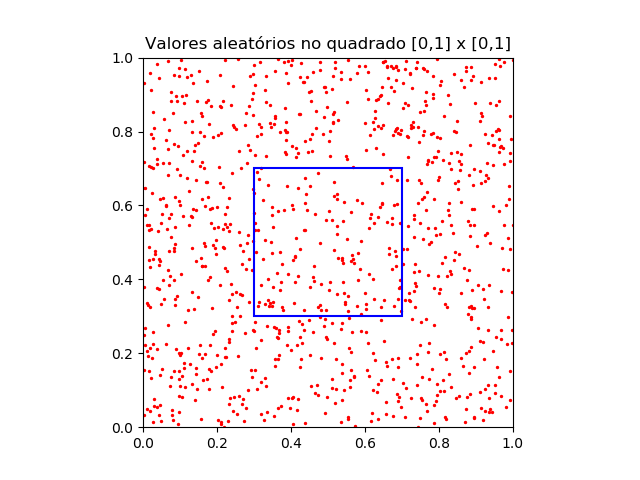
\includegraphics[scale=0.35]{pseudo10.png}
  \caption{Simulação Pseudo aleatória com 32 Pontos e 1024 pontos}
  \label{figura:32pseudo}
  \end{figure}
  
  
  \begin{figure}[h]
  \centering
  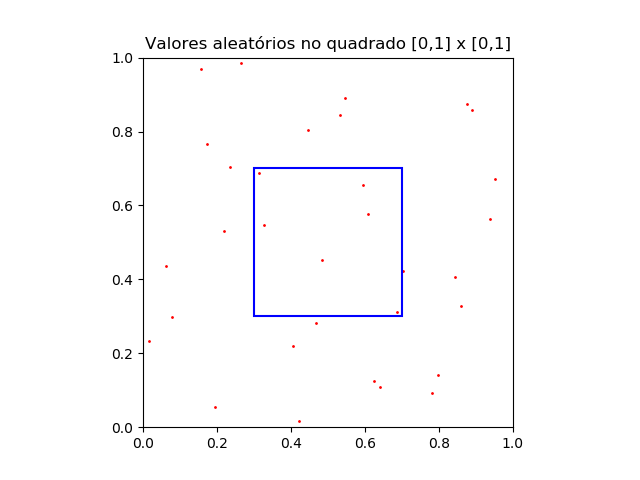
\includegraphics[scale=0.35]{quasi5.png} 
  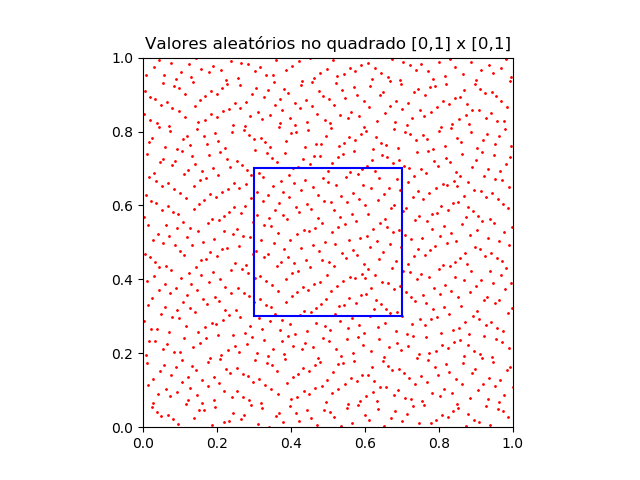
\includegraphics[scale=0.35]{quasi10.png}  
  \caption{Simulação Quasi aleatória com 32 pontos e 1024 pontos}
  \label{figura:quasi5}
  \end{figure}  

\textsc{MÉTODO}
\newline
 
  O método foi desenvolvido com linguagem python usando algumas funções básicas como a random para estar gerando os números pseudo aleatórios entre 0 e 1, uso do pacote MATPLOTLIB do python para gerar os gráficos e todas as imagens/configurações nescessárias para análise, enquanto que para os dados quasi-aleatórios foi usado funções que tomam como base a sequência SOBOL (A sequência de Sobol é mais simples que a Faure, pois, utiliza a base 2 para todas as dimensões, sendo portanto mais rápida, mas o procedimento de reordenação dos elementos dos vetores é mais complexo que a permutação utilizada em Faure, pois utiliza-se de um conjunto de números direcionais.(Glasserman,2004).
  Comparativamente às seqüências de Halton e Faure, a de Sobol é melhor tanto no que diz respeito ao tempo computacional expendido, quanto ao fato de que a perda de uniformidade da sequência acontece em uma dimensão d maior que 25).Foi indicado um número em torno de   100 simulações para N já determinado sendo inicialmente 32, 1 024, 32 768 e 1 000 000.\\
 
\textsc{SIMULAÇÕES }
\newline

 Com um certo número de pontos dentro do intervalo, e com base nesses valores e intervalo foi colocado dentro do mesmo um pequeno quadrado de dimensões $\frac{i}{10}, \frac{i+1}{10}, \frac{j}{10}, \frac{j+1}{10}$ com i,j variando entre 1 e 9, como ideia seria observar a relação entre o número de ocorrências dentro do quadrado interno e comparar com as pontos externos a ele de modo que se possa ter uma razão ou proporção de eventos para cada variação do número geral de pontos e tentar através de gráficos encontrar uma melhor curva ou reta que proporcione uma relação que se aproxime de $\frac{1}{\sqrt{n}}$ ou $\frac{ln(n)}{n}$  e que seja a melhor interpretação possivel sobre a relação conforme N cresce.\\
 
\textsc{CASO PSEUDO ALEATÓRIO}
\newline
  
 Através das primeiras simulações e gráficos adquiridos, para os valores pseudo-aleatórios e considerando as funções $\frac{1}{\sqrt{n}}$ e $\frac{ln(n)}{n}$ como base pois apresentam de certo modo um bom e rápido decaimento, observamos que possuem uma certa relação de modo que conforme o número de pontos distribuídos aumenta a razão ($\sum_{k=1}^{N}\frac{p_i}{N}$) entre pontos no quadrado interno e no quadrado [0,1] parece estar a se aproximar dos valores do gráfico da função $\frac{ln(n)}{n}$, enquanto que para poucos pontos distribuídos ocorre uma variação que não segue de forma muito proxima nenhuma das funções mencionadas acima pois ocorrem muitas variações entre pontos.Essa visualização pode ser melhorada ao pensarmos como uma equação de reta como por exemplo $(y = m * x + b + error)$ que pode estar ajustando de melhor forma alguma caracteristica dos pontos e as funções como por exemplo se analisar o possível valor esperado da variação dos pontos com base nas funções separadamente.
 
  Ou observar qual a correlação dos pontos entre si com as funções por meio do coeficiente de Pearson de modo que se estiver mais próximo de 1 ou -1 temos uma correlação forte caso contário, ou seja mais próximo de zero é baixa a correlação entre os dados, assim sendo  pouco provável de existir pontos que são equivalentes em cada conjunto de dados e desse modo podendo apresentar uma maior variabilidade, algo que vemos junto a função $\frac{1}{\sqrt{n}}$ que apresenta pontos pouco relacionados em sua volta ao contrario da outra função que apresenta algo direcionado a  duas vezes  uma certa relação de valores de modo que tem menos variabilidade conforme N aumenta.\\
  
\textsc{CASOS QUASI ALEATÓRIOS}
\newline

Diferente do que foi observado no caso Pseudo aleatório os pontos nesse segundo método ficam mais organizandos (Figura 2)  e melhor distribuidos mesmo que o N seja grande desse modo podemos analisar o caso como algo que possui variabilidade um pouco maior em relação ao caso anterior,  pelo motivo que os pontos vão estar se comportando de forma uniforme e que não precisam de tanta velocidade para chegar a menor variação possivel , pois essa relação apresenta também certa uniformidade o que mantem os pontos mais dispersos, ao contrário dos pseudo aleatórios que apresentam mudanças bem visíveis decaindo rápido.Por essa razão se observa pela regressão que os pontos seguem mais correlação com o gráfico da função $\frac{1}{\sqrt{n}}$ mesmo de todos os valores sejam baixos, ele está presente e são o suficientes para chegar a essa conclusão sobre variabilidade de que sua expressão de decaimento é mais lenta.\\
  
\textsc{CONCLUÇÃO}
\newline

   Após observar os gráficos de cada distribuição para os dados N pontos e M simulações se obtem como solução para descrever a variabilidade dos pontos dentro do quadrado [0,1] como algo que conforme aumentamos o número de eventos, se torna próximo de algo linear, de modo que temos pouca diferença entre pontos para ambas as simulações quandi N é grande, o que pode ser observado na correlação entre os tipos de eventos, do qual  chegamos em algo bem próximo do linear com coeficiente de correlação práximo de 1 o que significa que os pontos estão quase que ocorrendo em mesma proporção dentro do intervalo, e que tentem a seguir  a mesma relação com base nas funções base de decaimento ou seja uma das situações ocorre de certo modo mais próxima as algo ligado a função  $\frac{1}{\sqrt{n}}$ que não é tão rápida quanto a expressão logaritma, mas pelas simulações os dados tinham certo direcionamento para esse caso como pode ser visto nos gráficos de correlação entre os métodos e as funções tomadas como base, sendo apenas  a velocidade de  decaimento que as difere de modo que se observa que a variabilidade de uma situação sofre mais para chegar no ponto de equilibrio entre ambos os casos.\\
  
\textsc{OBSERVAÇÕES}
\newline
 Dos códigos desenvolvidos foram enviados 3 arquivos, sendo que 2 temos a simulação indivudual para cada caso com seus respectivos gráficos de correlação e de visualização da distribuição e o terceiro é a apresentada a comparação entre os modelos pseudo e quasi, de modo que podemos ver que conforme N cresce temos maior semelhança entre as variações de pontos. Para uso de correção dos programas foi fixado um total de 10 simulações pois cada gráfico aparece em cada interação podendo ser alterado no comando while<10 e no número de pontos no vet[ ] dentro dos laços.  
\section{Anexos gráficos de algumas simulações} 
  \begin{figure}[h]
  \centering
  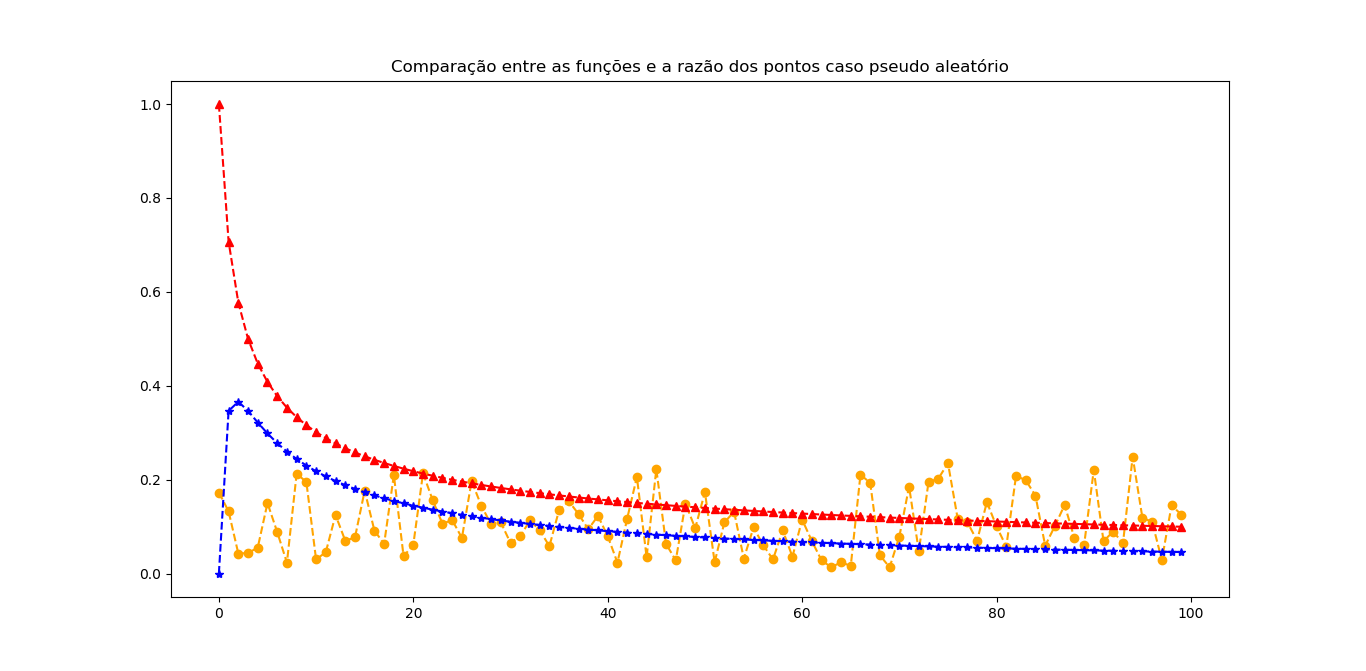
\includegraphics[scale=0.40]{pseudografi.png}
  \caption{Simulação Pseudo aleatória  da razão dos pontos em relação as funções  $\frac{ln(n)}{n}$   (azul) e $\frac{1}{\sqrt{n}}$ (vermelho)}
  \label{figura:pseudografi}
  \end{figure}


 \begin{figure}[h]
  \centering
  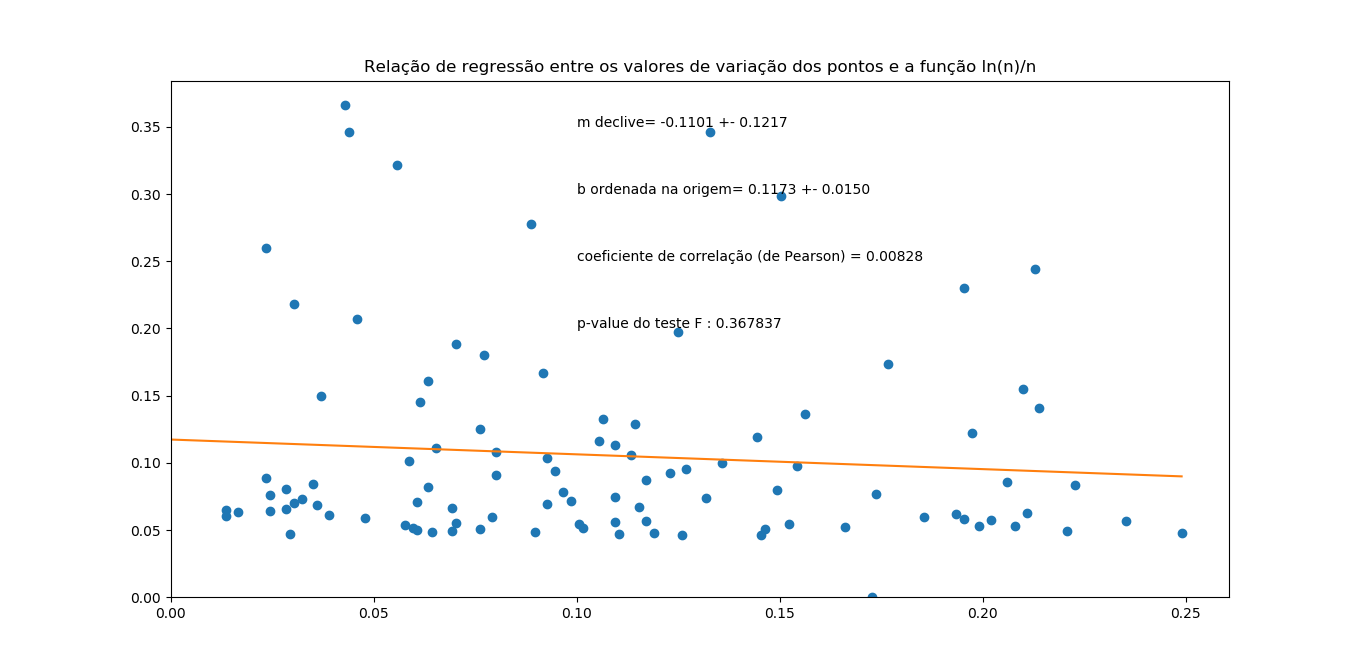
\includegraphics[scale=0.40]{reglnpseudo.png}
  \caption{Regressão que compara correlação no caso pseudo aleatório para função $\frac{ln(n)}{n}$}
  \label{figura:reglnpseudo}
  \end{figure} 
    
    
  \begin{figure}[h]
  \centering
  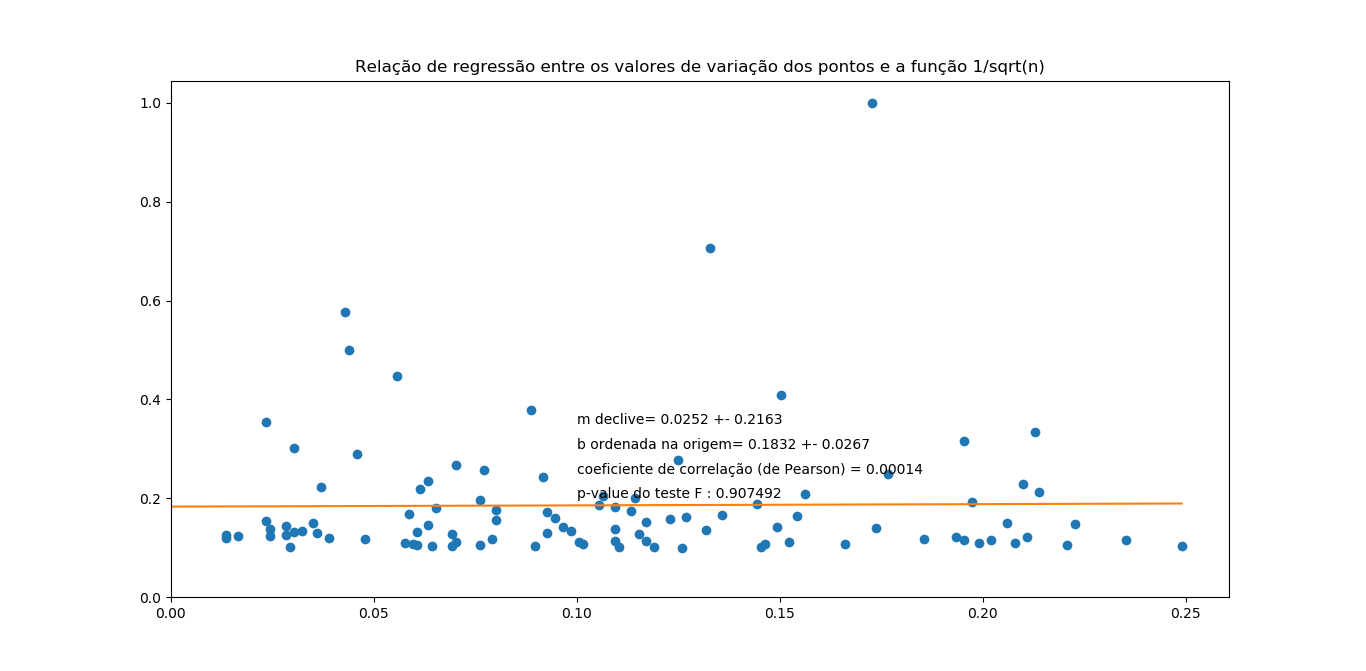
\includegraphics[scale=0.40]{reg1sqrtpseudo.png}
  \caption{Regressão que compara correlação  no caso pseudo aleatório para função  $\frac{1}{\sqrt{n}}$}
  \label{figura:reg1sqrtpseudo}
  \end{figure}
    
  \begin{figure}[h]
  \centering
  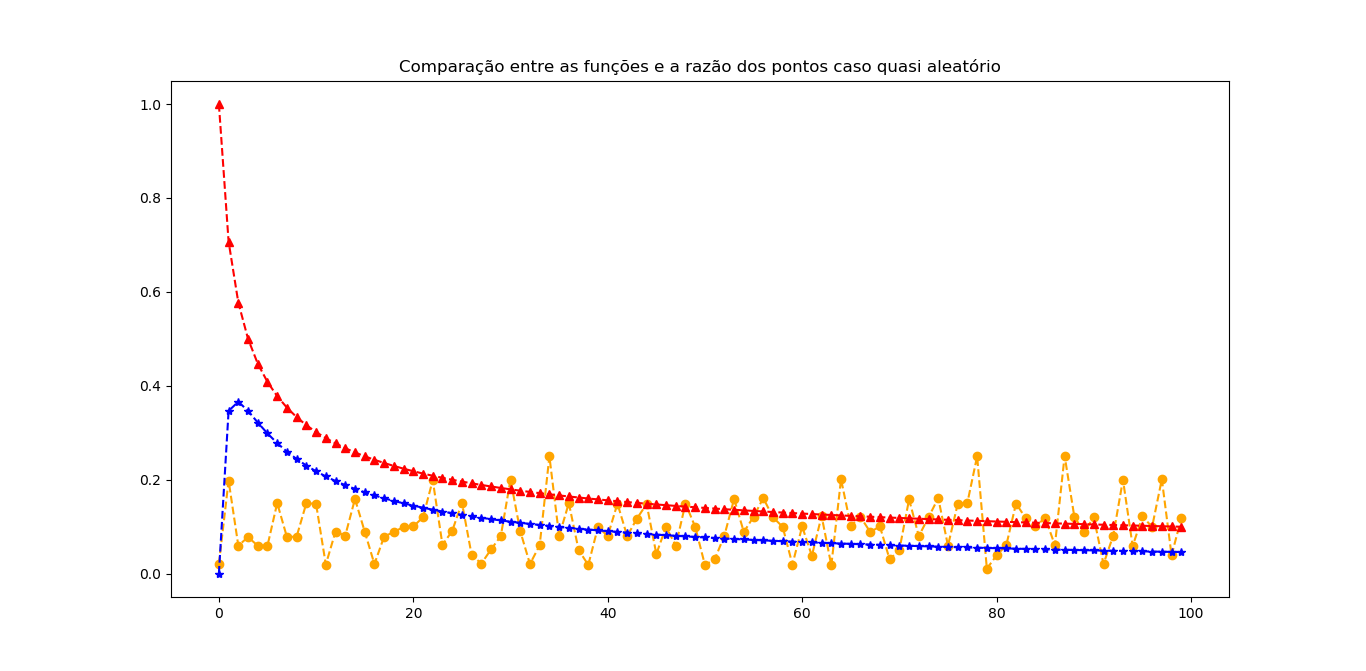
\includegraphics[scale=0.40]{graficospontosquasi.png}
  \caption{Simulação Quasi aleatória  da razão dos pontos em relação as funções  $\frac{ln(n)}{n}$ (azul) e $\frac{1}{\sqrt{n}}$ (vermelho)}
  \label{figura:graficospontosquasi}
  \end{figure}
 
  
  \begin{figure}[h]
  \centering
  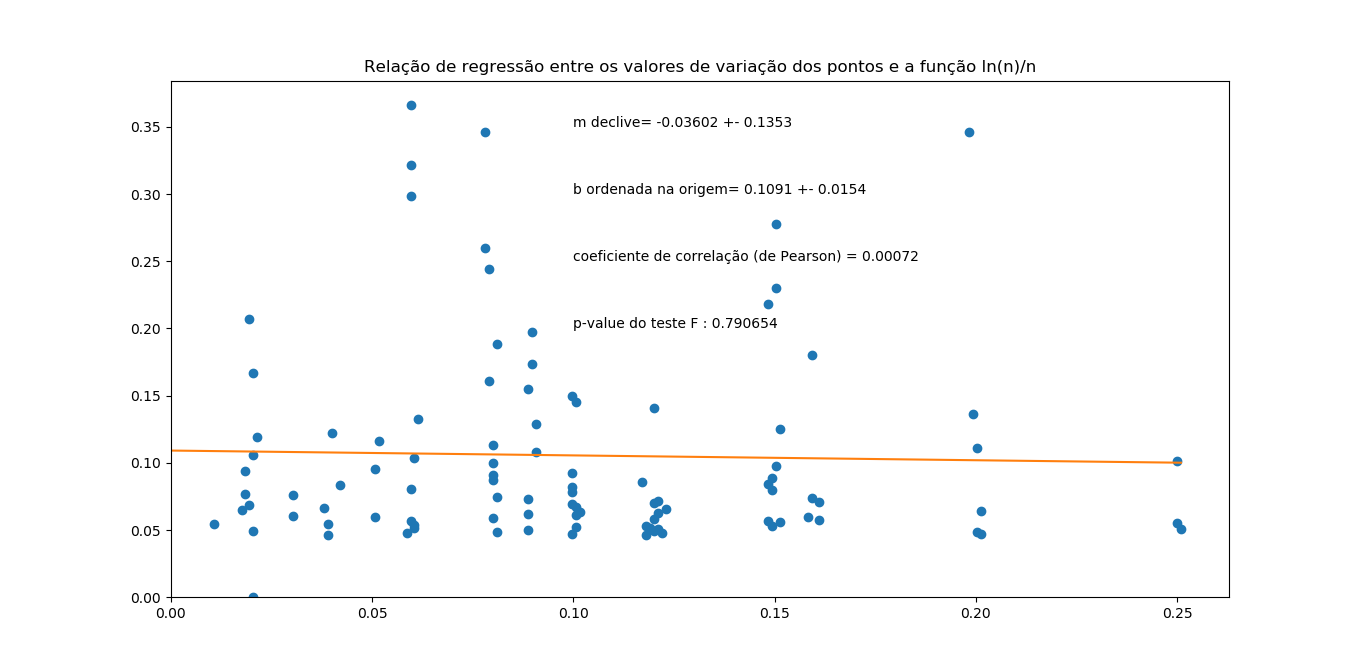
\includegraphics[scale=0.40]{regrecaoln.png}
  \caption{Regressão que compara correlação no caso quasi aleatório para função $\frac{ln(n)}{n}$}
  \label{figura:regrecaoln}
  \end{figure}
  
  \begin{figure}[h]
  \centering
  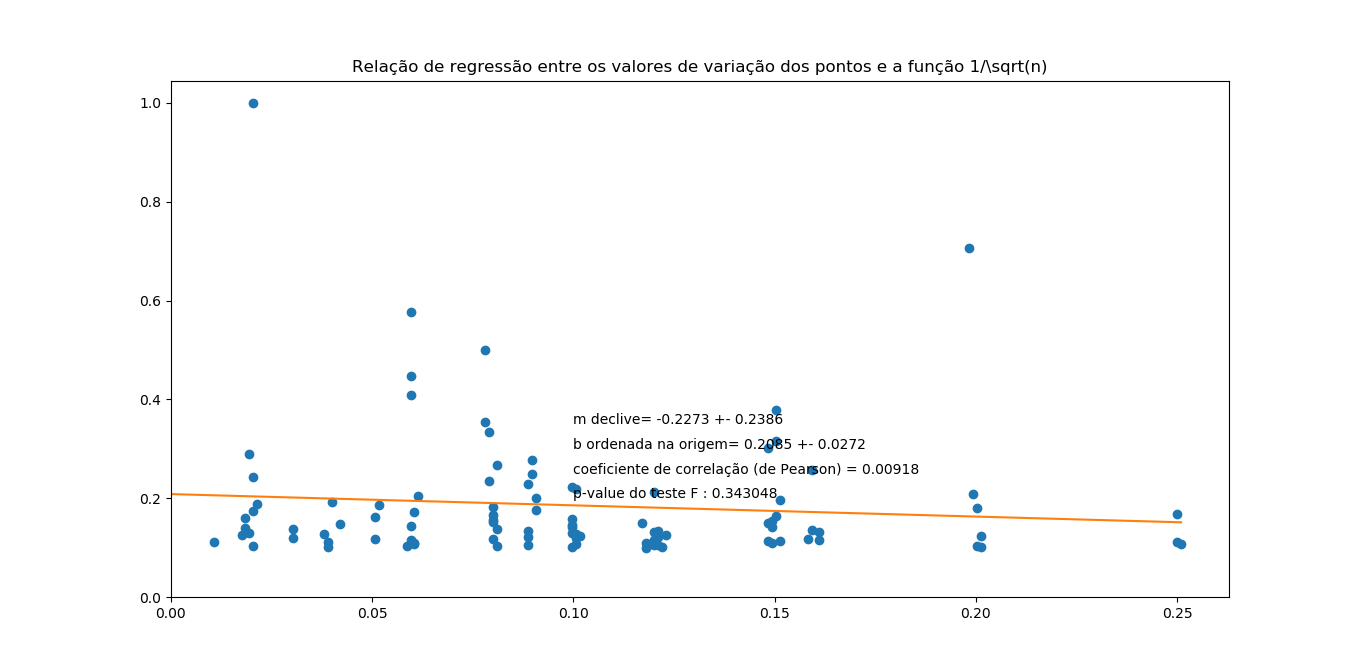
\includegraphics[scale=0.40]{regrecao1sqrt.png}
  \caption{Regressão que compara correlação no caso quasi aleatório para função  $\frac{1}{\sqrt{n}}$}
  \label{figura:regrecao1sqrt}
  \end{figure}
  
  
   \begin{figure}[h]
  \centering
  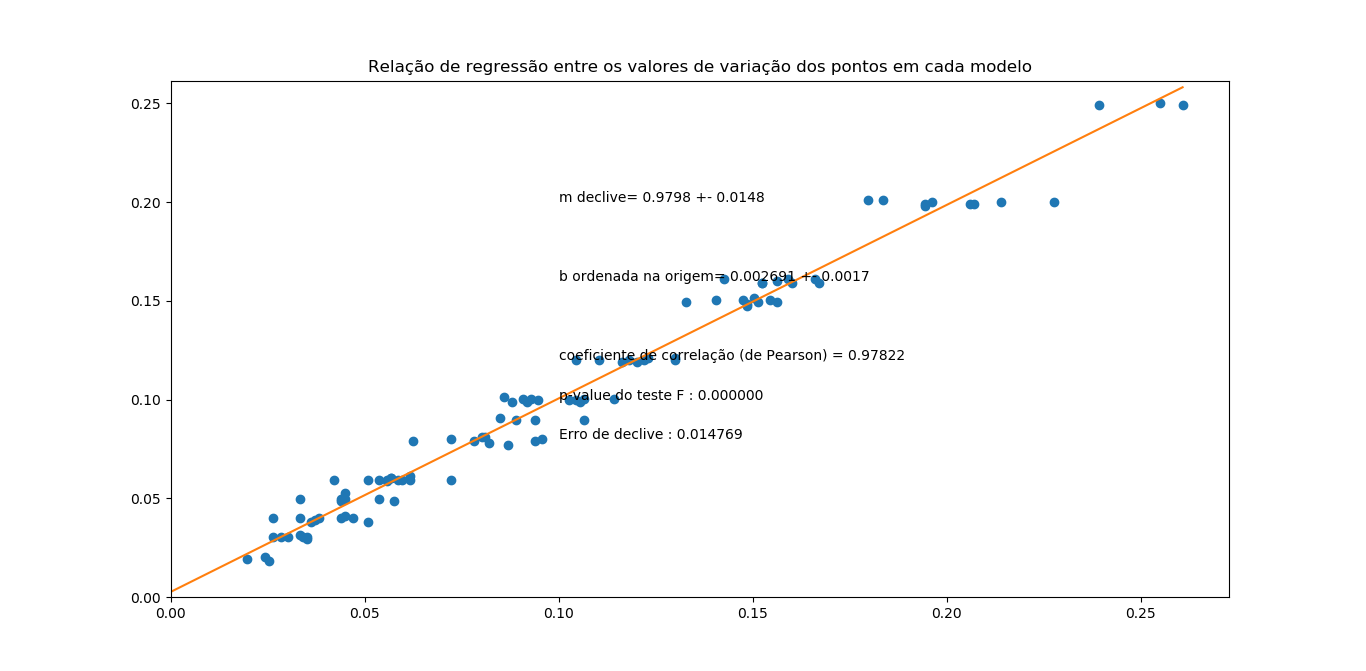
\includegraphics[scale=0.40]{regreentrecasos.png}
  \caption{Comparando valores de correlação entre os pontos quasi e pseudo aleatórios}
  \label{figura:regreentrecasos}
  \end{figure} 
  
  
\end{document}